\subsection{The Cherenkov Telescope Array}
\begin{frame}{The Cherenkov Telescope Array}
  \begin{minipage}{0.48\textwidth}
    \begin{itemize}
      \item Three telescope types: SST, MST, LST
      \item Energy range coverage from $\SI{20}{\giga\eV}$ up to $\SI{300}{\tera\eV}$
      \item Two sites: CTA south (Atacama Desert, Chile), CTA north (La Palma, Spain)
    \end{itemize}
  \end{minipage}
  \begin{minipage}{0.48\textwidth}
    \centering
    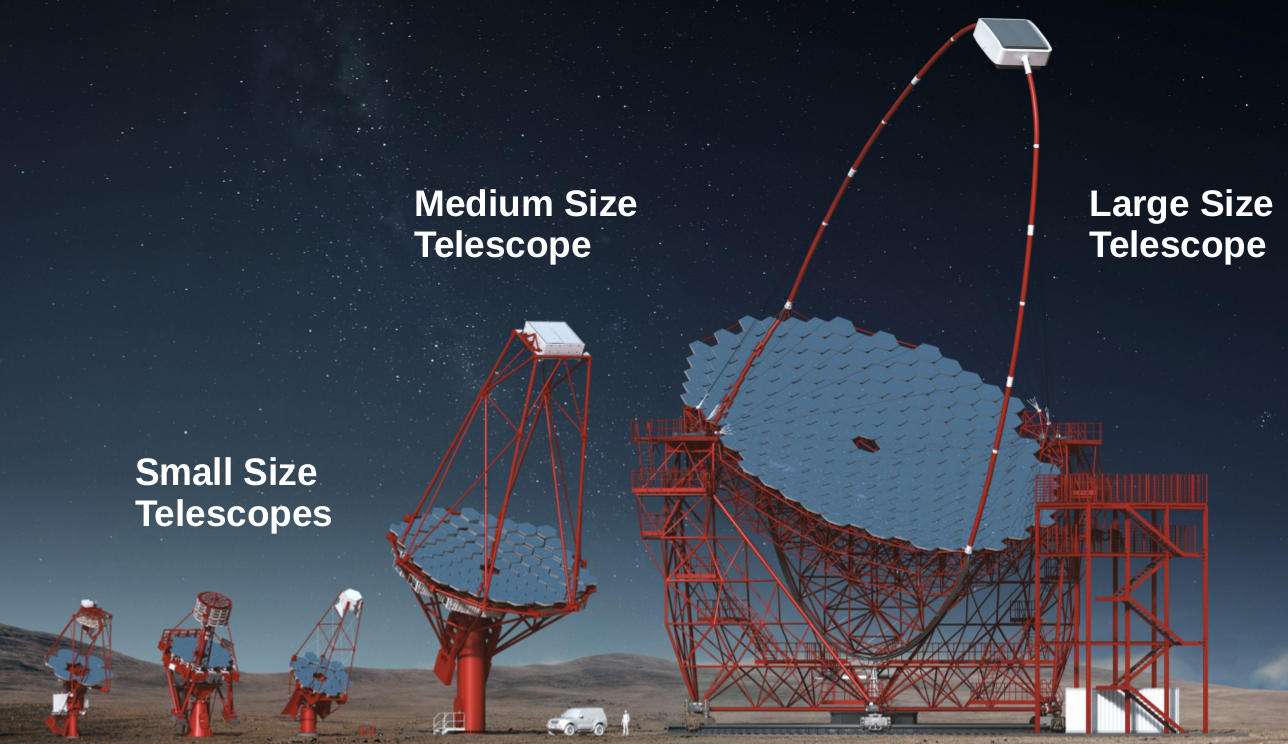
\includegraphics[width=\textwidth]{graphics/imagetelescope.png}
  \end{minipage}
\end{frame}


\subsection{Transients}
\begin{frame}{Transients}
  TESTETSTETSETET
  \begin{itemize}
    \item Astronomical event lasting from seconds to weeks, sometimes years
    \begin{itemize}
      \item [\to] Very short compared to the timescales in which the galaxies or the universe formed
    \end{itemize}
    \item Transient events include: Gamma-ray bursts, novae, gravitional waves, etc.
  \end{itemize}
\end{frame}
